\documentclass[a4paper,11]{article} 
\usepackage[left=1in,right=1in,top=2cm,bottom=2cm]{geometry}
\usepackage{graphicx}
\usepackage{subcaption}
\usepackage{float}
\usepackage{listings}
\usepackage{color}
\usepackage{amsmath}
\usepackage{hyperref}

\graphicspath{{../data/}{../data/results/}}
\hypersetup{colorlinks=true,linkcolor=blue,urlcolor=blue}
  
\definecolor{codegreen}{rgb}{0,0.6,0}
\definecolor{codegray}{rgb}{0.5,0.5,0.5}
\definecolor{codepurple}{rgb}{0.58,0,0.82}
\definecolor{backcolour}{rgb}{0.95,0.95,0.92}
 
\lstdefinestyle{mystyle}{
    backgroundcolor=\color{backcolour},   
    commentstyle=\color{codegreen},
    keywordstyle=\color{magenta},
    numberstyle=\tiny\color{codegray},
    stringstyle=\color{codepurple},
    basicstyle=\footnotesize,
    breakatwhitespace=false,         
    breaklines=true,                 
    captionpos=t,                    
    keepspaces=true,                 
    numbers=left,                    
    numbersep=5pt,                  
    showspaces=false,                
    showstringspaces=false,
    showtabs=false,                  
    tabsize=4
}
 
\lstset{style=mystyle}
\pagenumbering{gobble}
\allowdisplaybreaks

\begin{document}

\begin{center}
  \large{\textbf{CSE578 Computer Vision}}\\
  \Large{\textbf{Assignment 2 : Image Mosaicing}}\\
  \vspace{1em}
  Karnik Ram\\
  2018701007
\end{center}

The procedure for image mosaicing, along with the code is explained in this report. The generated results are provided at the end. The code files are provided in the \texttt{src} directory along with this submission.

The code is written in C++ and is written as a class (\texttt{Panaroma}) for modularity. The class is explained with comments in the file \texttt{panaroma.h}. To run the program,

\begin{lstlisting}[language=bash]
mkdir build && cd build
cmake ..
make
./run <image1-path> <image2-path> [<image3-path> ...]  <ouput-mosaic-path>
# eg: ./run ../data/img1_1.png ../data/img1_2.png ../data/results/mosaic1.png
\end{lstlisting}

The program is scalable to any number of input images, of any size. However, overlap must exist between any image in the sequence and one or more of the previous images in the sequence.


\section{Procedure with Code}
Each step in the procedure is explained briefly in the following subsections, along with the corresponding code.
  \subsection{Keypoints detection and matching}
  
  In order to estimate the homography between any pair of images, we first need pairs of corresponding points from both the images. This is obtained using OpenCV's SIFT implementation.
  \begin{figure}[H]
    \centering
    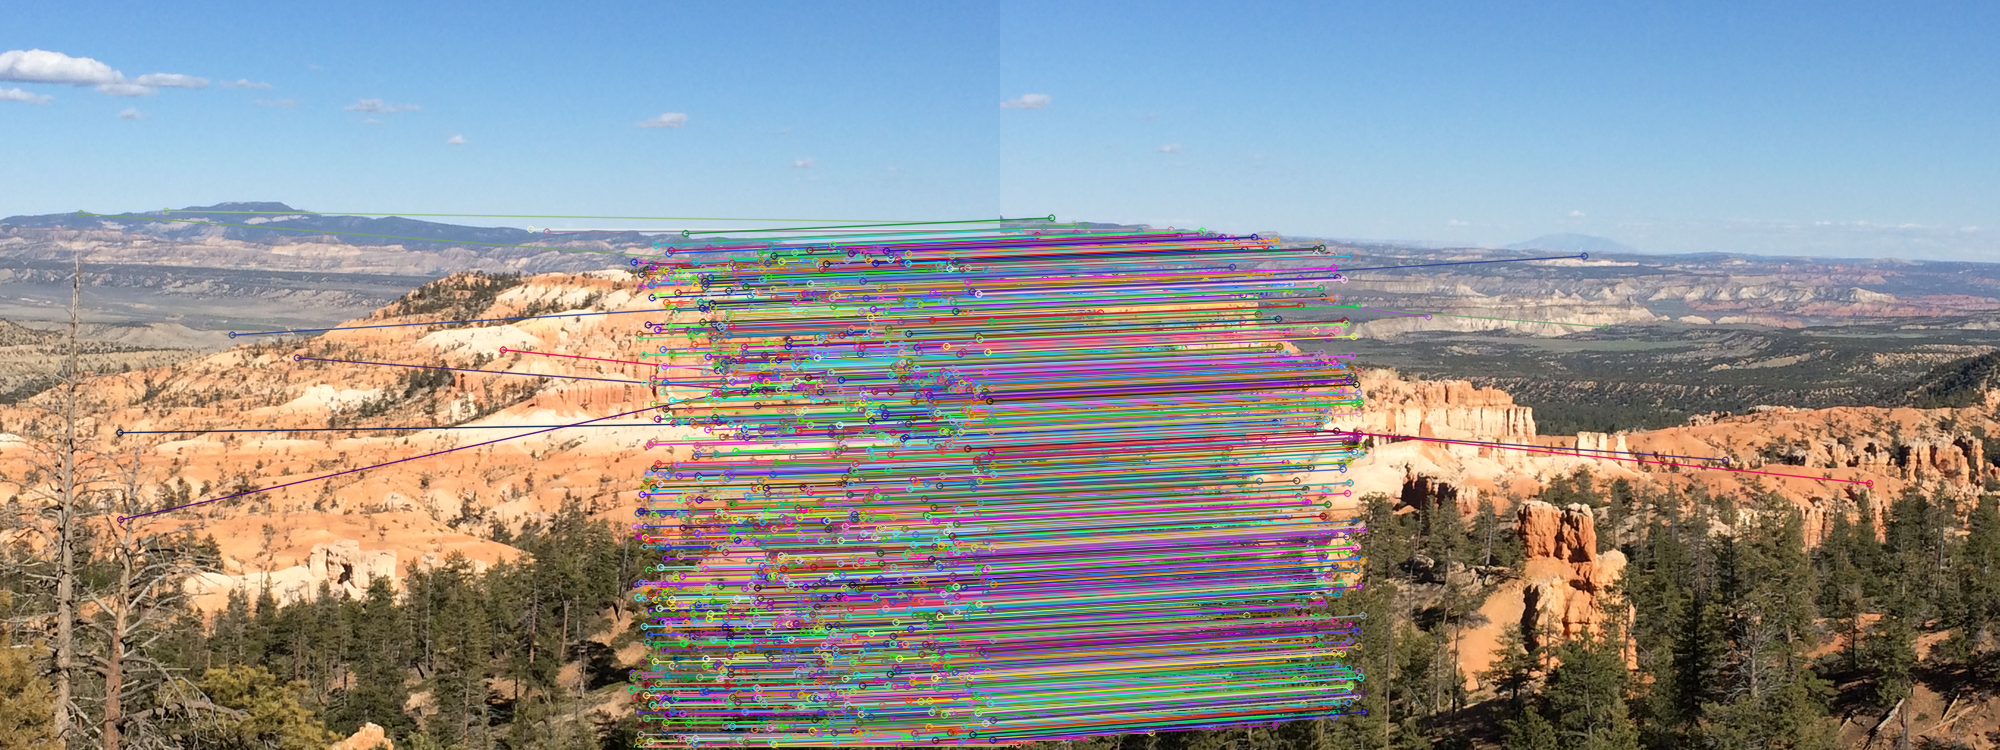
\includegraphics[width=0.8\linewidth]{sift-eg}
    \caption{Keypoints detected and matched using SIFT feature descriptors and nearest-neighbor based matching in OpenCV.}
  \end{figure}

  
  \noindent The following is the corresponding code:
  \begin{lstlisting}[language=C++]
void Panaroma::generateMatches(const cv::Mat &img1, const cv::Mat &img2,
    	Eigen::MatrixXf &X1, Eigen::MatrixXf &X2, const int &id)
{
    cv::Ptr<cv::xfeatures2d::SIFT> detector = cv::xfeatures2d::SIFT::create();
    std::vector<cv::KeyPoint> keypoints1, keypoints2;
    cv::Mat descriptors1, descriptors2;

    //Detection and description
    detector->detectAndCompute(img1, cv::noArray(), keypoints1, descriptors1);
    detector->detectAndCompute(img2, cv::noArray(), keypoints2, descriptors2);

    //Matching
    cv::Ptr<cv::DescriptorMatcher> matcher = cv::DescriptorMatcher::create(cv::DescriptorMatcher::FLANNBASED);
    std::vector< std::vector<cv::DMatch> > knn_matches;
    matcher->knnMatch( descriptors1, descriptors2, knn_matches, 2 );

    //Refine matches using Lowe's ratio threshold
    const float ratio_thresh = 0.7f;
    std::vector<cv::DMatch> good_matches;
    for(size_t i = 0; i < knn_matches.size(); i++)
    {
        if (knn_matches[i][0].distance < ratio_thresh * knn_matches[i][1].distance)
        {
            good_matches.push_back(knn_matches[i][0]);
        }
    }

    cv::Mat img_matches;
    cv::drawMatches(img1, keypoints1, img2, keypoints2, good_matches, img_matches, cv::Scalar::all(-1),
        cv::Scalar::all(-1), std::vector<char>(), cv::DrawMatchesFlags::NOT_DRAW_SINGLE_POINTS);
    cv::imshow("Good Matches " + std::to_string(id), img_matches);
    std::cout << "Number of matches found: " << good_matches.size() << std::endl;

    //Store corresponding points in homogeneous representation
    X1.resize(good_matches.size(),2);
    X2.resize(good_matches.size(),2);

    size_t j = 0;
    for(cv::DMatch match : good_matches)
    {
	    cv::Point2f pt = keypoints1[match.queryIdx].pt;
	    X1(j,0) = pt.x;
	    X1(j,1) = pt.y;

	    pt = keypoints2[match.trainIdx].pt;
	    X2(j,0) = pt.x;
	    X2(j++,1) = pt.y;
    }

    X1.conservativeResize(X1.rows(),X1.cols()+1);
    X2.conservativeResize(X1.rows(),X2.cols()+1);

    X1.col(X1.cols()-1).setOnes();
    X2.col(X2.cols()-1).setOnes();
}

  \end{lstlisting}
  \vspace{1em}
  
  \subsection{Robust Homography estimation}
  
    Using the corresponding points, the homography is then estimated using the DLT algorithm.
    
    \noindent The code as follows:
    \begin{lstlisting}[language=C++]
void Panaroma::estimateHomography(const Eigen::MatrixXf &X1, const Eigen::MatrixXf &X2,
    	Eigen::MatrixXf &H)
{
	Eigen::MatrixXf A(2*X1.rows(), 9);
	Eigen::ArrayXf h(9);

	for(int i = 0, j = 0; i < A.rows(); i+=2, j++)
	{
		A.row(i) << 0, 0, 0, -1 * X2(j,2) * X1.row(j), X2(j,1) * X1.row(j);
		A.row(i+1) << X2(j,2) * X1.row(j), 0, 0, 0, -1 * X2(j,0) * X1.row(j);
	}

	// This gave bad results for some unknown reason
	//Eigen::JacobiSVD<Eigen::MatrixXf> svd(A,Eigen::ComputeThinU | Eigen::ComputeThinV);

	cv::Mat cv_A,U,S,Vt;
	eigen2cv(A,cv_A);
	cv::SVD::compute(cv_A,U,S,Vt);

	Eigen::MatrixXf V,tempV;
	cv2eigen(Vt,tempV);
	V = tempV.transpose();

	h = V.col(V.cols()-1);

	H.resize(3,3);
	H.row(0) = h.segment(0,3);
	H.row(1) = h.segment(3,3);
	H.row(2) = h.segment(6,3);

	std::cout << "H:\n" << H << std::endl;
}\end{lstlisting}
    \vspace{1em}
    
    \begin{figure}
    \centering
    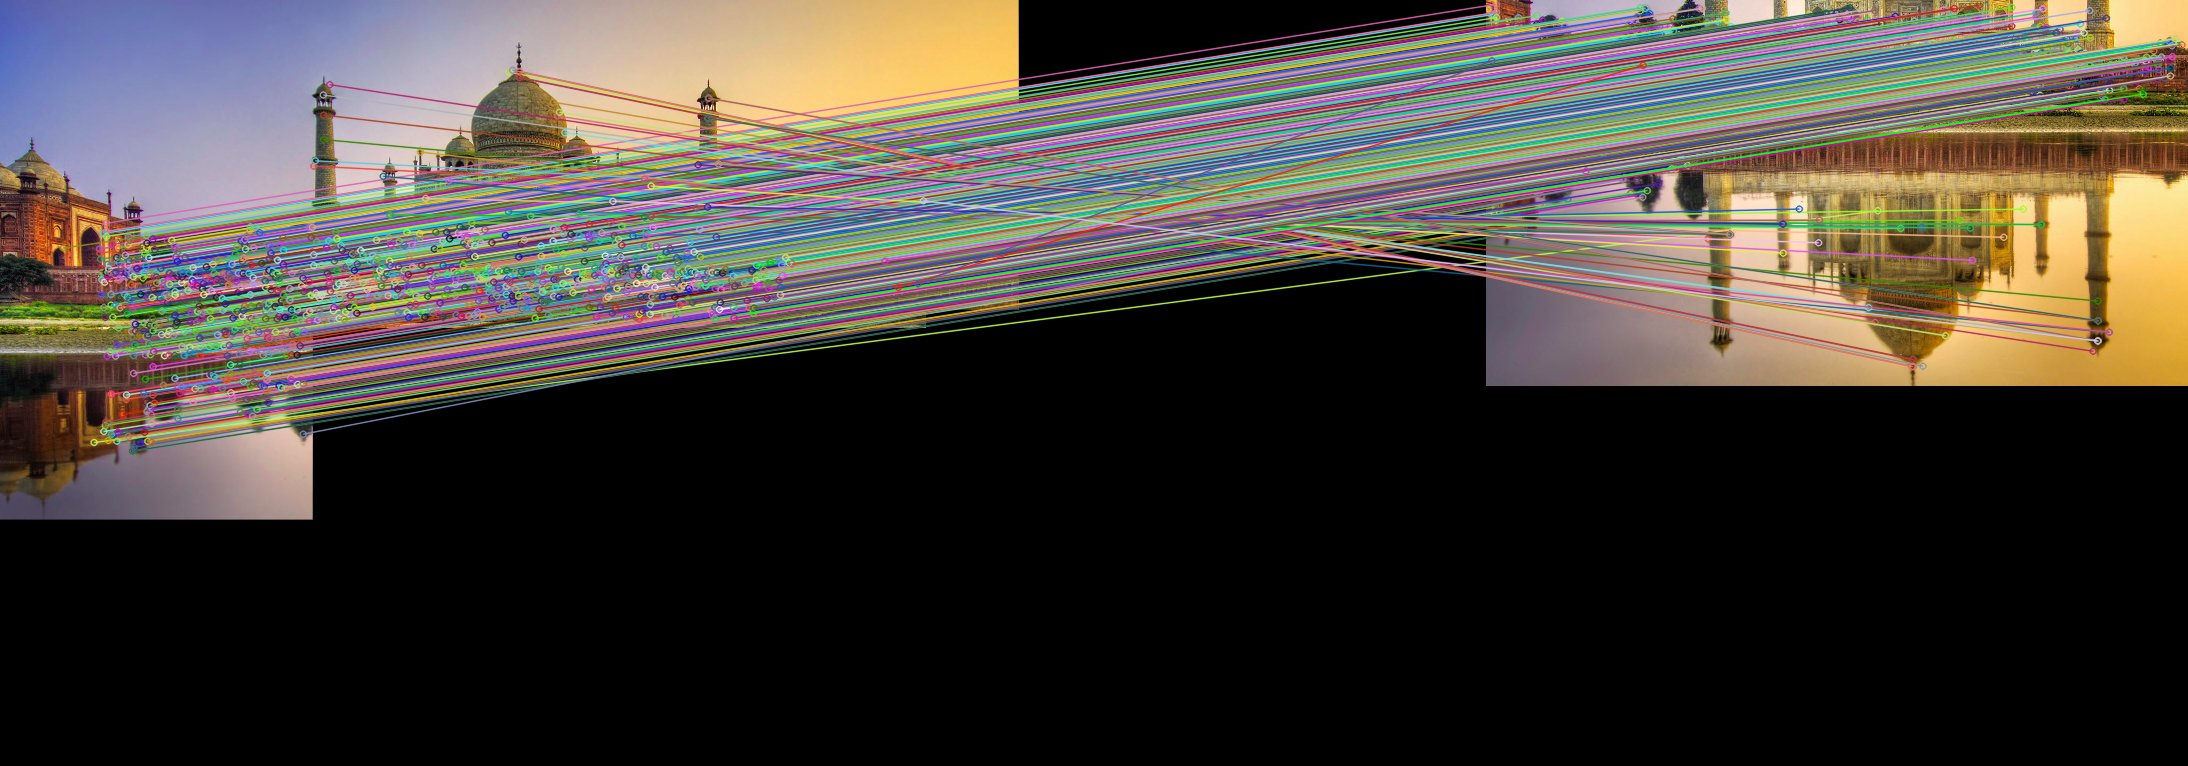
\includegraphics[width=0.8\linewidth]{h-robust}
    \caption{The matching process gives some outliers as shown. The homography is estimated within a RANSAC scheme to take care of this.}
  \end{figure}
  
  However, the esimated homography will be noisy due to the presence of outliers from the matching process. To take care of this, homography is estimated within a RANSAC scheme.
  
  \noindent The correspoding code is as follows:
    \begin{lstlisting}[language=C++]
void Panaroma::estimateRansacHomography(const Eigen::MatrixXf &X1, const Eigen::MatrixXf &X2,
		const float &dist_threshold, const float &ratio_threshold, Eigen::MatrixXf &H,
		std::vector<int> &inlier_indices)
{
	std::cout << "Estimating Homography within RANSAC..." << std::endl;
	Eigen::MatrixXf sample_X1, sample_X2;
	Eigen::Vector3f x1,x2;
	std::vector<int> largest_support;
	float inlier_avg = 0;

	for(size_t i = 0; i < 2000; i++)
	{
		std::cout << "\n\nIteration#" << i+1 << std::endl;
		std::vector<int> sample_indices = utils::generateRandomVector(0,X1.rows()-1,4);

		sampleFromX1X2(X1,X2,sample_indices,sample_X1,sample_X2);
		estimateHomography(sample_X1,sample_X2,H);

		for(size_t j = 0; j < X1.rows(); j++)
		{
			if(std::find(sample_indices.begin(),sample_indices.end(),j) != sample_indices.end())
				continue;

			x1 = X1.row(j);
			x2 = X2.row(j);

			if( calcReprojectionError(x1,x2,H) <= dist_threshold )
			{
				inlier_indices.push_back(j);
				inlier_avg += calcReprojectionError(x1,x2,H);
			}
		}

		std::cout << "\nNumber of inliers: " << inlier_indices.size() << std::endl;
		std::cout << "Inlier avg. reprojecion error: " << inlier_avg / inlier_indices.size() << std::endl;
		inlier_avg = 0;

		if(inlier_indices.size() >= X1.rows() * ratio_threshold)
		{
			std::cout << "\nFound a model!\nNumber of inliers: " << inlier_indices.size() << std::endl;
			inlier_indices.insert(inlier_indices.end(),sample_indices.begin(),sample_indices.end());
			sampleFromX1X2(X1,X2,inlier_indices,sample_X1,sample_X2);
			estimateHomography(sample_X1,sample_X2,H);
			std::cout << "Original number of SIFT matches: " << X1.rows() << std::endl;
			std::cout << "Average reprojection error over inliers and sample set: " << calcAvgReprojectionError(sample_X1,sample_X2,H) << std::endl;
			return;
		}

		else
		{
			if(largest_support.size() < inlier_indices.size())
			{
				largest_support = inlier_indices;
				largest_support.insert(largest_support.end(),sample_indices.begin(),sample_indices.end());
			}

			inlier_indices.clear();
		}
	}

	if(largest_support.size() >= 4)
	{
		std::cout << "\nCould not find a model according to threshold!\nSo using largest inlier set instead." << std::endl;
		sampleFromX1X2(X1,X2,largest_support,sample_X1,sample_X2);
		estimateHomography(sample_X1,sample_X2,H);
		inlier_indices = largest_support;
		std::cout << "Number of inliers: " << largest_support.size() << std::endl;
		std::cout << "Original number of SIFT matches: " << X1.rows() << std::endl;
		std::cout << "Average reprojection error over inliers and sample set: " << calcAvgReprojectionError(sample_X1,sample_X2,H) << std::endl;
	}

	else
		std::cout << "Could not find a model!" << std::endl;
}
    
    \end{lstlisting}
    \vspace{1em}
    
  \subsection{Image warping}
  
  Using the estimated homography, the second image is warped into the first image's frame. This is done as an inverse warping operation with bilinear interpolation. The image is also made twice as large as the original since the warped coordinates will extend outside the original plane.
  
    \begin{figure}[H]
    \centering
    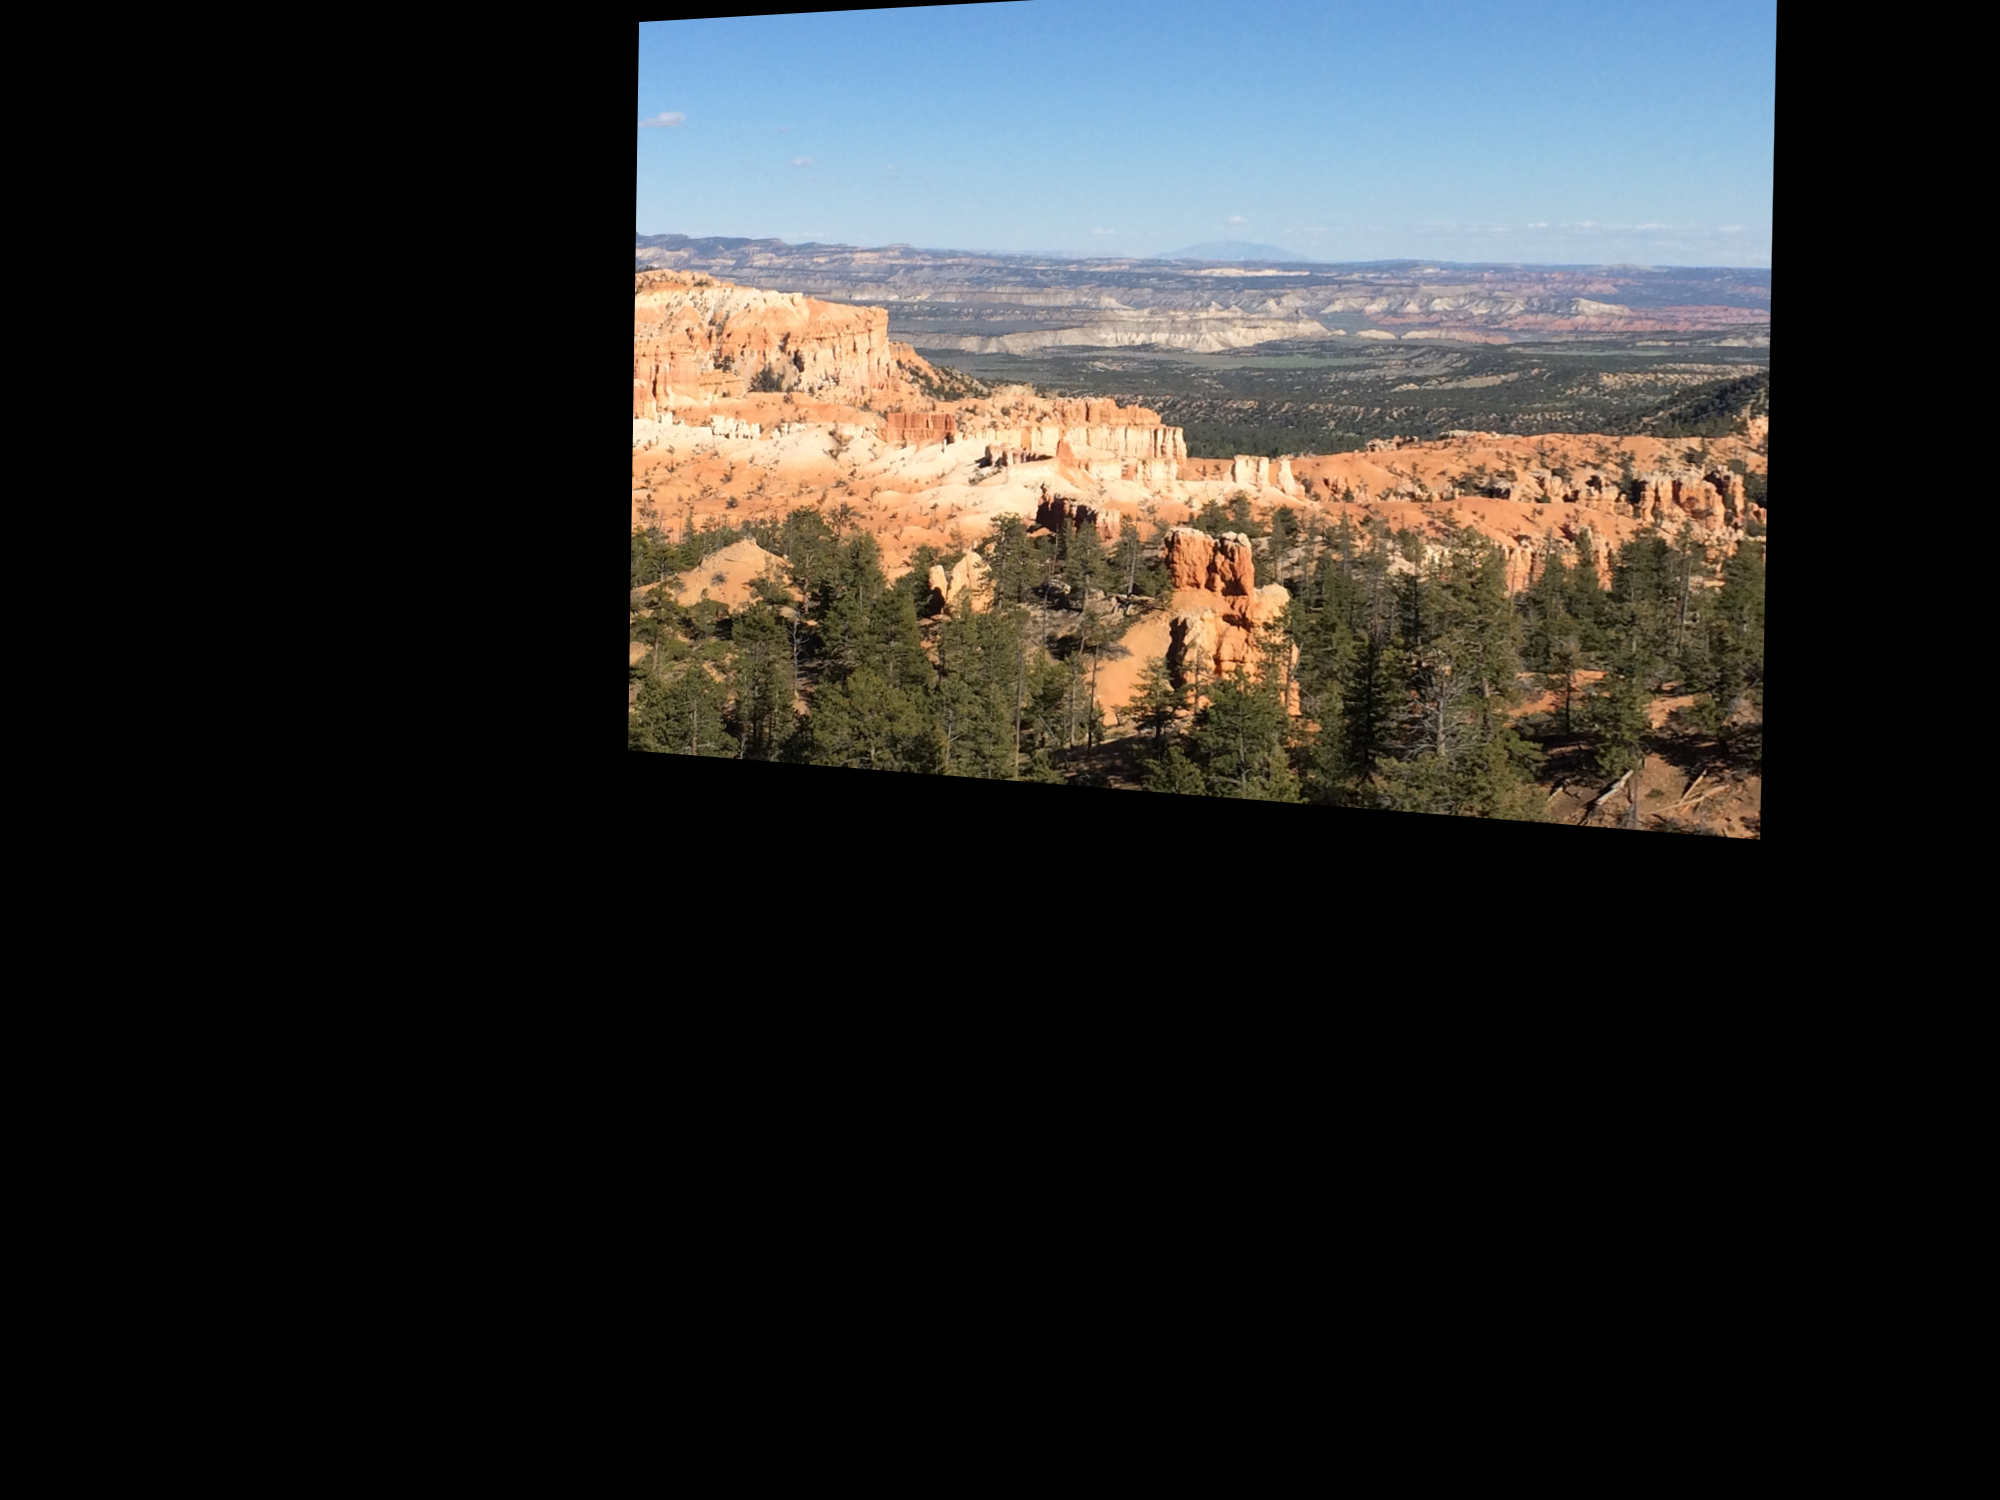
\includegraphics[scale=0.15]{warped-eg}
    \caption{The second image is warped into the first image's frame using the estimated homography.}
  \end{figure}
  
    \noindent The code is as follows:
    \begin{lstlisting}[language=C++]
void Panaroma::warpImage(cv::Mat src_img, const Eigen::Matrix3f &H, cv::Mat &warped_img)
{
	cv::Mat map_x, map_y;
	warped_img = cv::Mat::zeros(2*src_img.rows,2*src_img.cols,src_img.type());
	
	cv::hconcat(src_img,cv::Mat::zeros(src_img.size(),src_img.type()),src_img);
	cv::vconcat(src_img,cv::Mat::zeros(src_img.size(),src_img.type()),src_img);

	map_x.create(src_img.size(),CV_32FC1);
	map_y.create(src_img.size(),CV_32FC1);
	
	for(int i = 0; i < warped_img.rows; i++)
		for(int j = 0; j < warped_img.cols; j++)
		{
			Eigen::Vector3f x(j,i,1);
			Eigen::Vector3f px = H * x;
			px = px/px(2);

			map_x.at<float>(i,j) = px(0);
			map_y.at<float>(i,j) = px(1);
		}

	cv::remap(src_img,warped_img,map_x,map_y,CV_INTER_LINEAR);
} 
    \end{lstlisting}
    \vspace{1em}
  \subsection{Image stitching}
  
  The warped image is then aligned and added with the first image. The common regions are subtracted out from the first image before doing so.
  
    \begin{figure}[H]
    \centering
    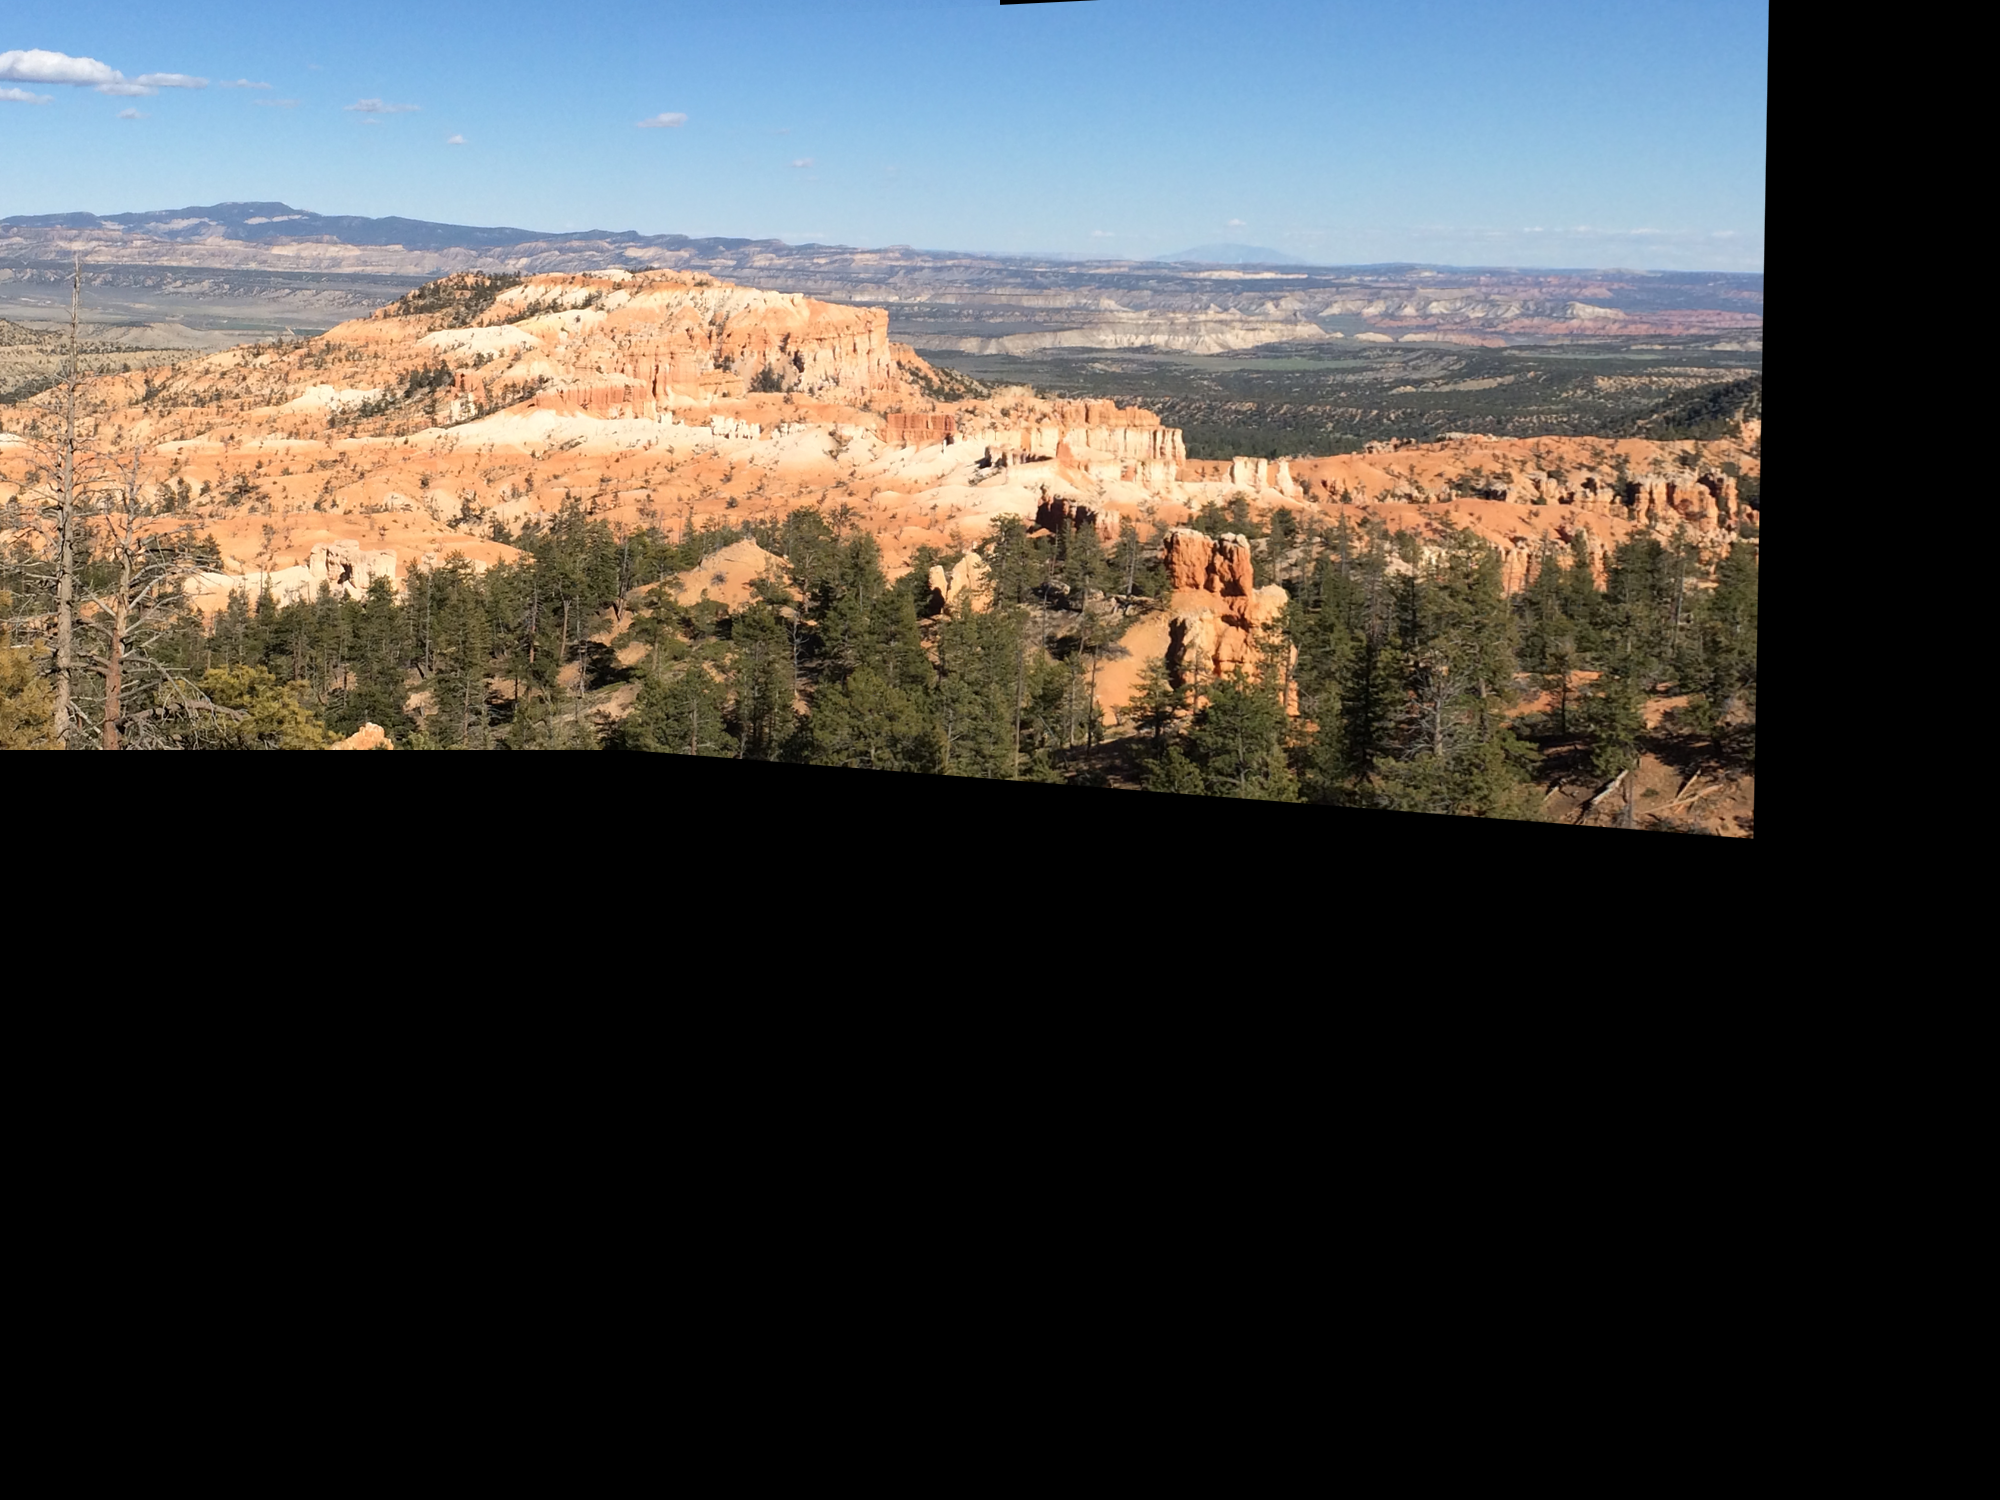
\includegraphics[scale=0.2]{mosaic1}
    \caption{The warped image is then added (and subtracted) onto the first image.}
  \end{figure}
  
    \begin{lstlisting}[language=C++]
void Panaroma::stitch(cv::Mat img1, cv::Mat img2, cv::Mat &result)
{
	int rows_offset, cols_offset;
	rows_offset = img1.rows - img2.rows;
	cols_offset = img1.cols - img2.cols;
    
    // To ensure both images are of same size
	if(rows_offset < 0)
		cv::vconcat(img1,cv::Mat::zeros(abs(rows_offset),img1.cols,img1.type()),img1);
	
	else if(rows_offset > 0)
		cv::vconcat(img2,cv::Mat::zeros(abs(rows_offset),img2.cols,img2.type()),img2);

	if(cols_offset < 0)
		cv::hconcat(img1,cv::Mat::zeros(img1.rows,abs(cols_offset),img1.type()),img1);

	else if(cols_offset > 0)
		cv::hconcat(img2,cv::Mat::zeros(img2.rows,abs(cols_offset),img2.type()),img2);

	cv::Mat temp;
	cv::subtract(img1,img2,temp);
	cv::add(temp,img2,result);
}
    \end{lstlisting}
    \vspace{2em}
  \subsection{Loop over multiple Images}
  
  This process is then repeated for the next images in the sequence. The generated mosaic is taken as the new first image, and the next image is matched with it and a new mosaic is again generated, and so on.
   
    \begin{lstlisting}[language=C++]
void Panaroma::run(const float &dist_threshold, const float &ratio_threshold)
{
	Eigen::MatrixXf X1,X2, H;
    std::vector<int> inlier_indices;
    cv::Mat warped_image, mosaic;

	generateMatches(images[0],images[1],X1,X2,0);
   	estimateRansacHomography(X1,X2,dist_threshold,ratio_threshold,H,inlier_indices);
   	warpImage(images[1],H,warped_image);
 	stitch(images[0],warped_image,mosaic);

	X1.resize(0,0);
	X2.resize(0,0);
	inlier_indices.clear();

	for(size_t i = 2; i < images.size(); i++)
	{
		generateMatches(mosaic,images[i],X1,X2,i);
   		estimateRansacHomography(X1,X2,dist_threshold,ratio_threshold,H,inlier_indices);
	   	warpImage(images[i],H,warped_image);
 		stitch(mosaic,warped_image,mosaic);
		X1.resize(0,0);
		X2.resize(0,0);
		inlier_indices.clear();
	}

	cv::namedWindow("Mosaic",CV_WINDOW_NORMAL);
	cv::imshow("Mosaic",mosaic);
	cv::imwrite(output_path,mosaic);

	std::cout << "Output mosaic written to "<< output_path << " !" << std::endl;
    cv::waitKey(0);
}
    \end{lstlisting}
    \vspace{2em}
   
  
\section{Results}
All the input and generated images can also be found here - \href{https://drive.google.com/drive/folders/1yWDCrjAzcIT8lY5YrfEgnE_MRmjcgCXH?usp=sharing}{link}.
  \subsection{\texttt{img1} set}
  
  \begin{figure}[H]
    \begin{subfigure}{.5\textwidth}
      \centering
      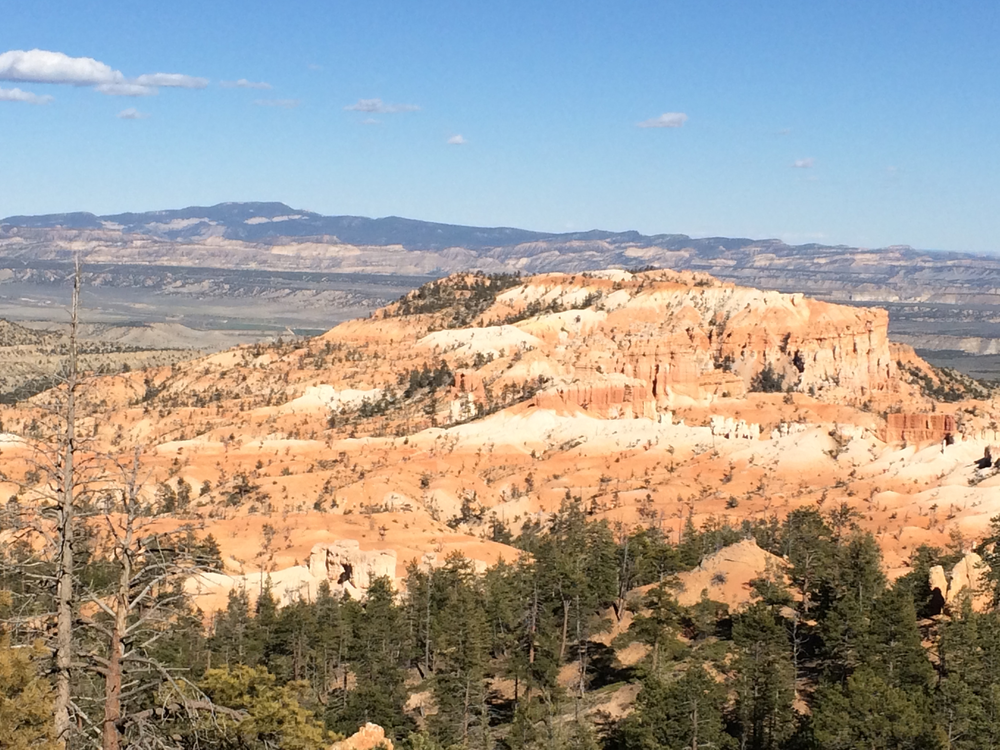
\includegraphics[width=.8\linewidth]{img1_1}
      \caption{Input 1}
    \end{subfigure}
    \begin{subfigure}{.5\textwidth}
      \centering
      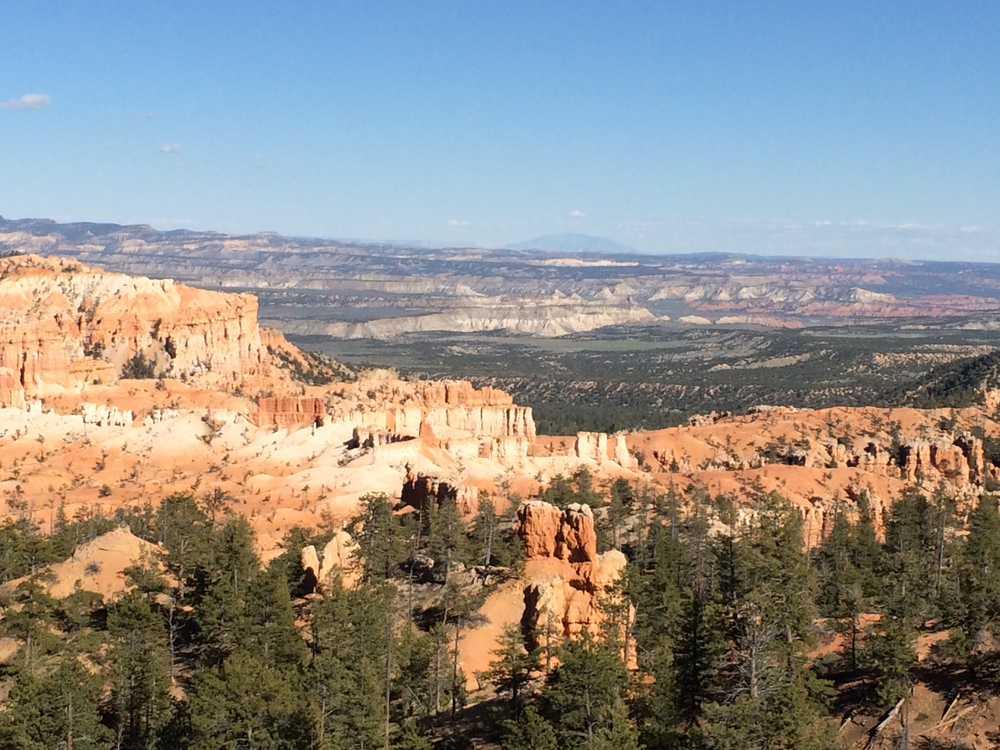
\includegraphics[width=.8\linewidth]{img1_2}
      \caption{Input 2}
    \end{subfigure}
    \begin{subfigure}{\textwidth}
      \centering
      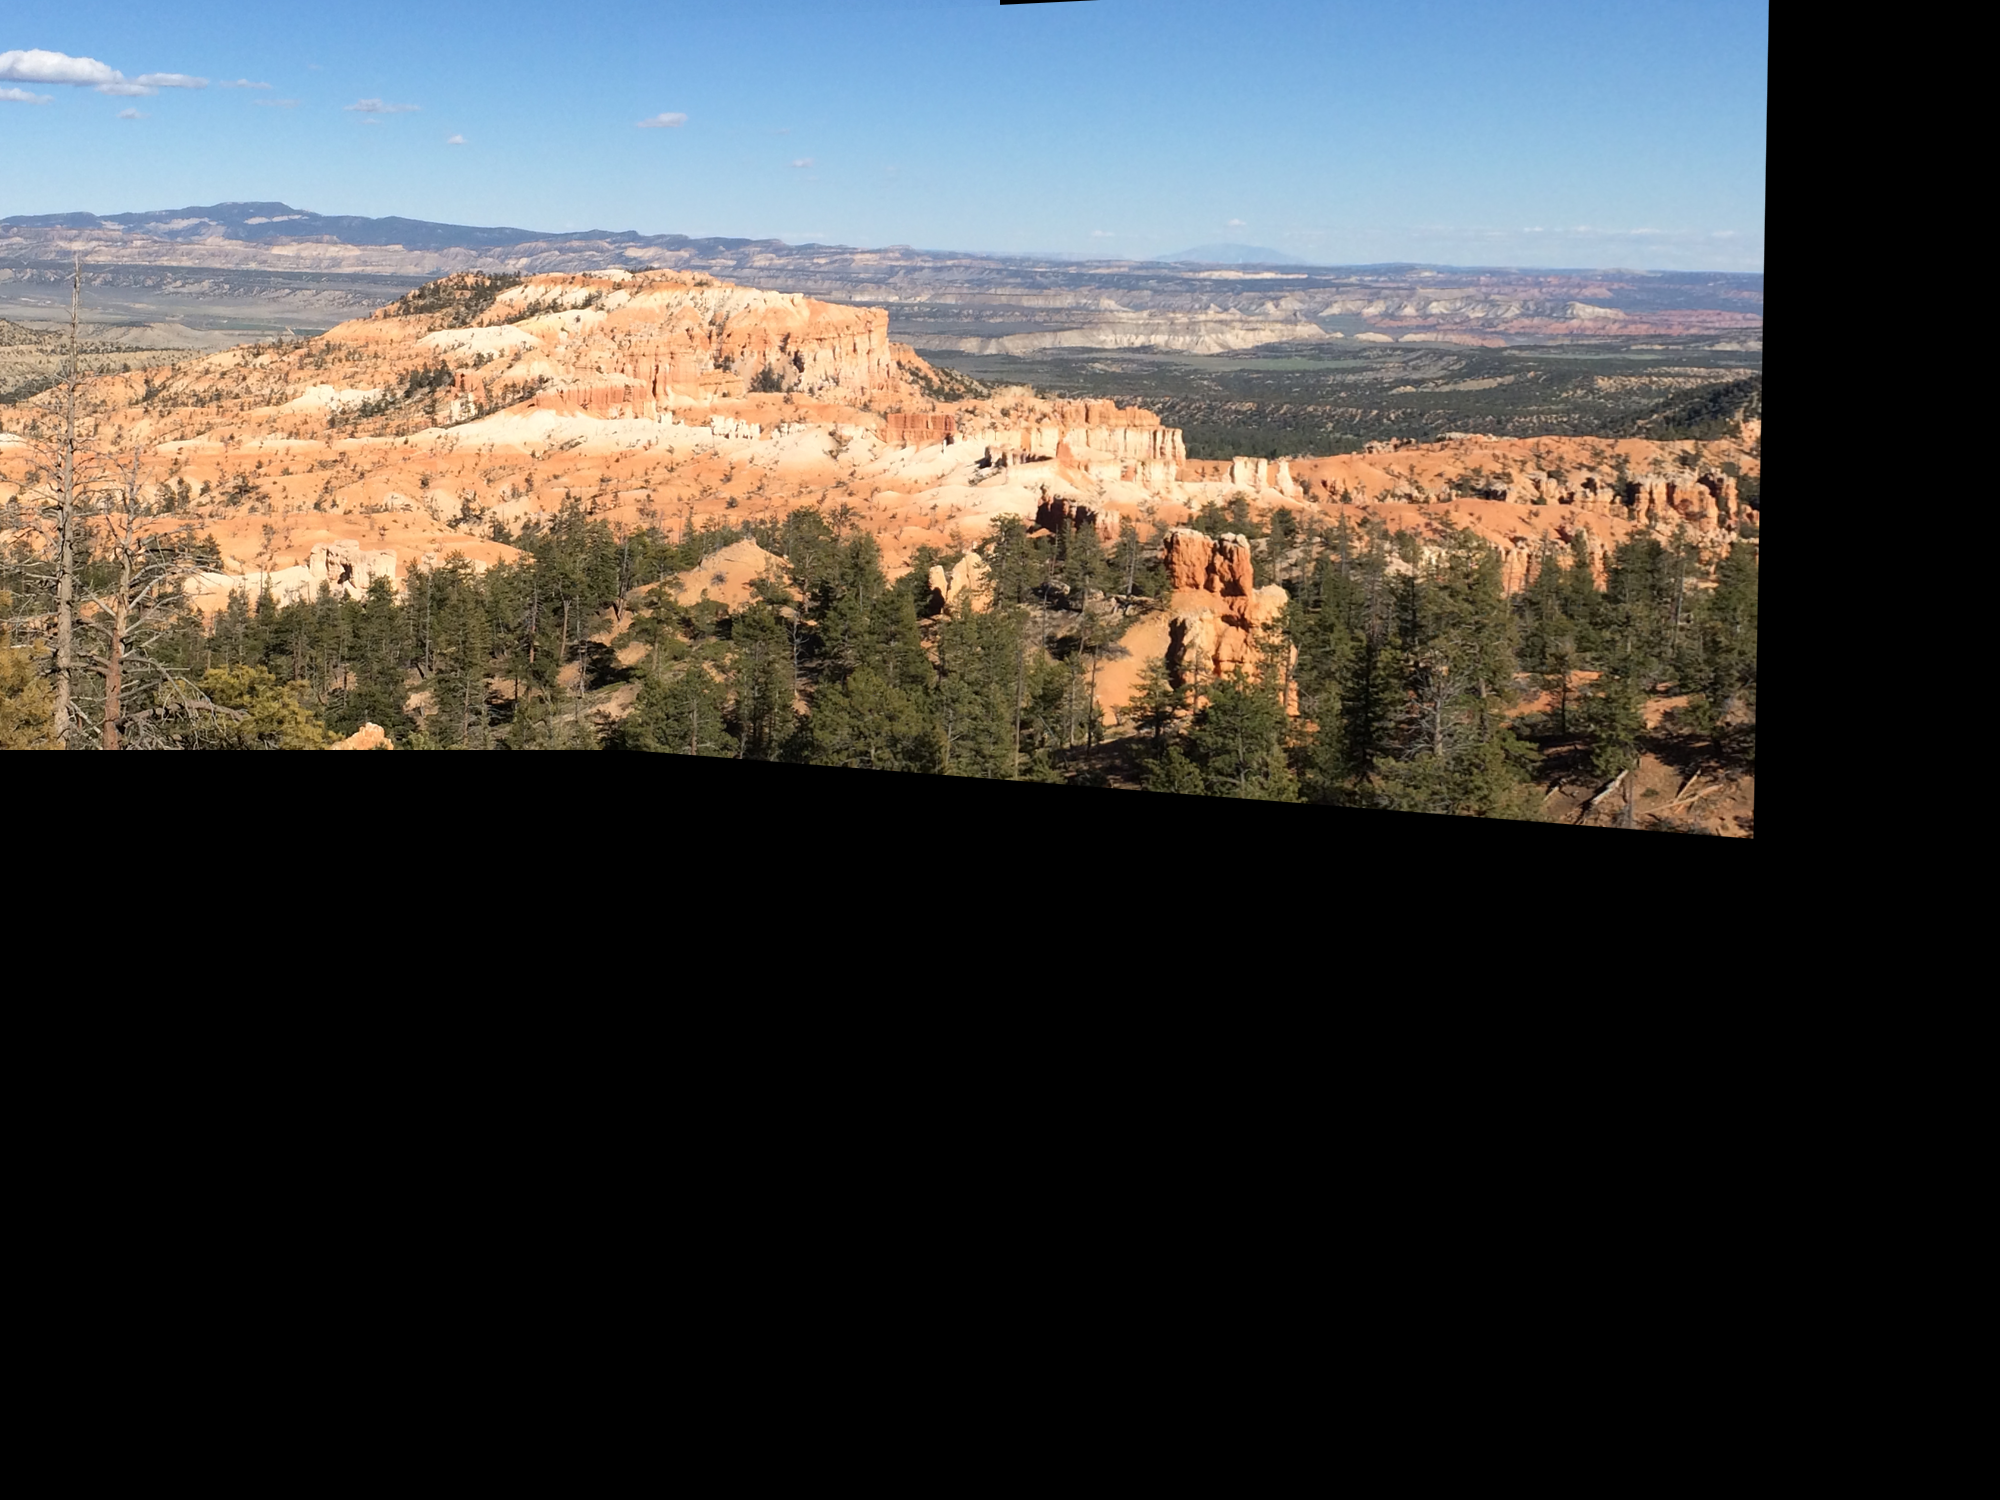
\includegraphics[width=.8\linewidth]{mosaic1}
      \caption{Result}
    \end{subfigure}
  \end{figure}

  
  \subsection{\texttt{img2} set}
    \begin{figure}[H]
      \begin{subfigure}{.5\textwidth}
	\centering
	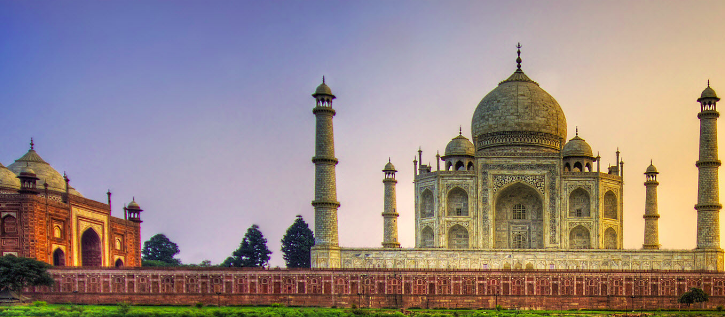
\includegraphics[width=.8\linewidth]{img2_1}
	\caption{Input 1}
      \end{subfigure}
      \begin{subfigure}{.5\textwidth}
	\centering
	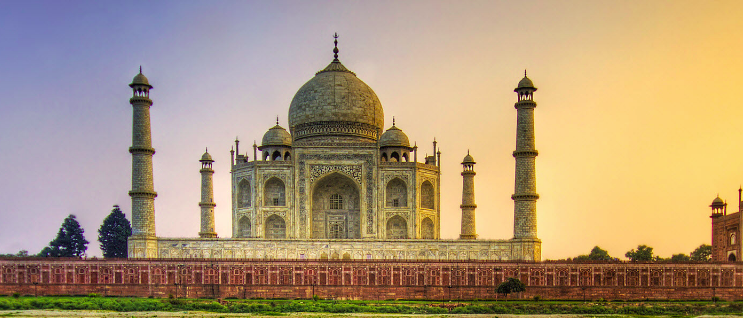
\includegraphics[width=.8\linewidth]{img2_2}
	\caption{Input 2}
      \end{subfigure}
      \end{figure}
      \begin{figure}\ContinuedFloat
      \begin{subfigure}{0.5\textwidth}
	\centering
	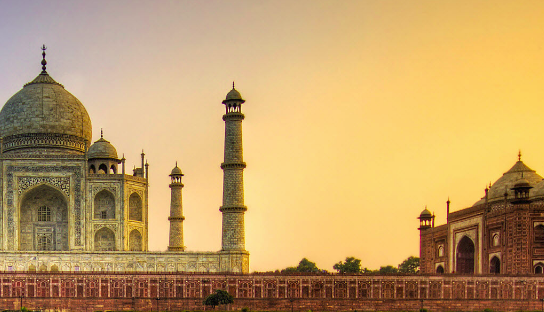
\includegraphics[width=.8\linewidth]{img2_3}
	\caption{Input 3}
      \end{subfigure}
      \begin{subfigure}{0.5\textwidth}
	\centering
	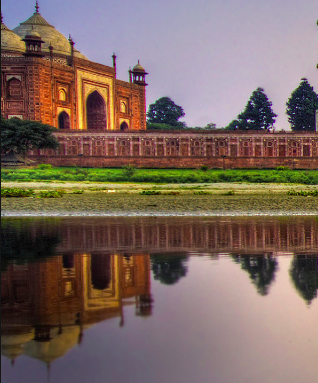
\includegraphics[width=.8\linewidth]{img2_4}
	\caption{Input 4}
      \end{subfigure}
      \begin{subfigure}{0.5\textwidth}
	\centering
	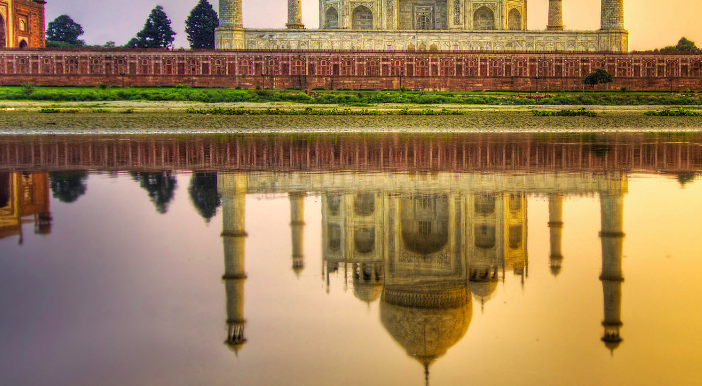
\includegraphics[width=.8\linewidth]{img2_5}
	\caption{Input 5}
      \end{subfigure}
      \begin{subfigure}{0.5\textwidth}
	\centering
	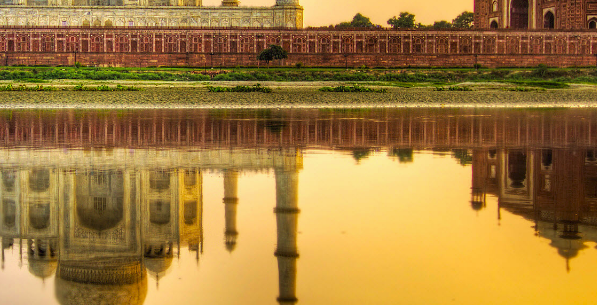
\includegraphics[width=.8\linewidth]{img2_6}
	\caption{Input 6}
      \end{subfigure}
      \begin{subfigure}{\textwidth}
	\centering
	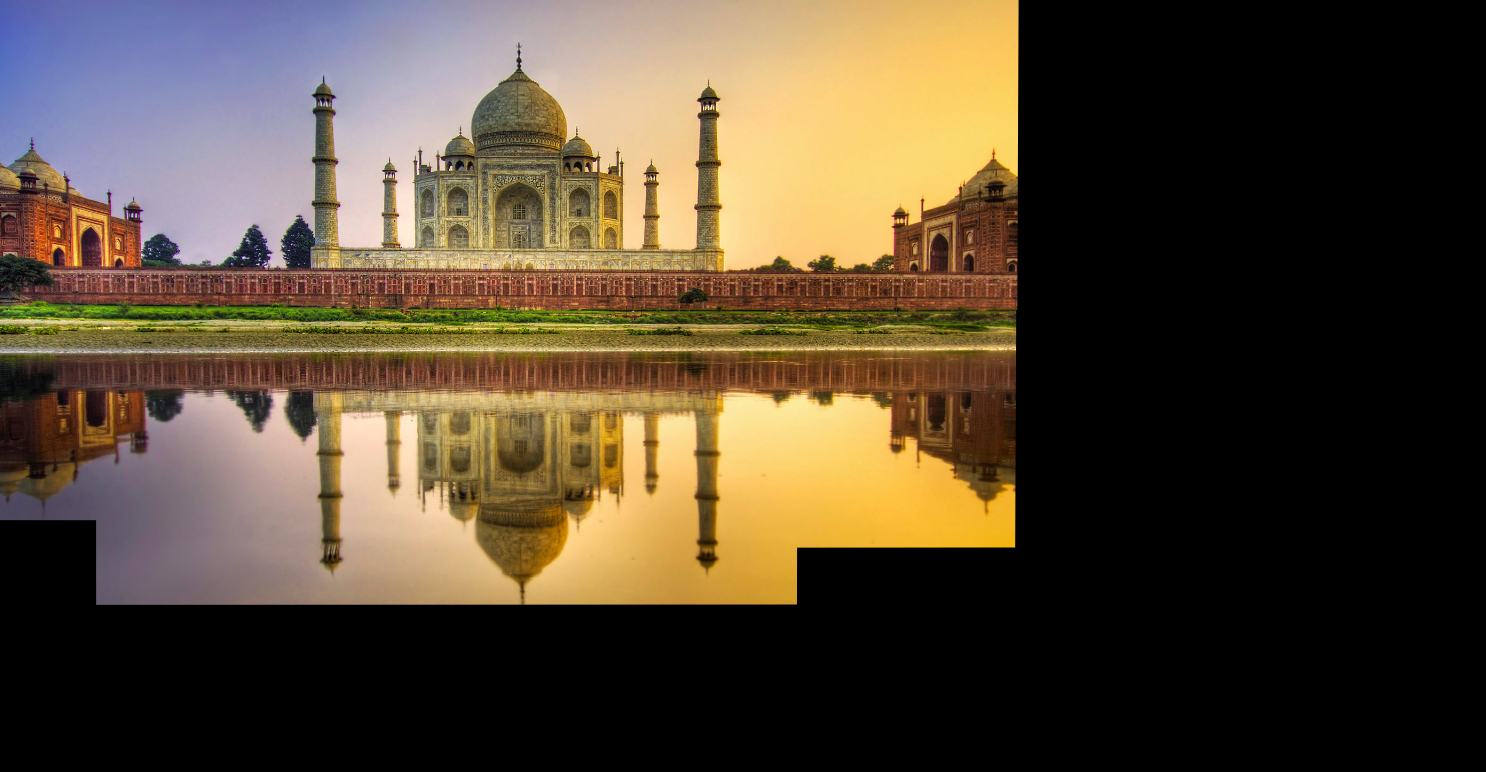
\includegraphics[width=.8\linewidth]{mosaic2}
	\caption{Result}
      \end{subfigure}
    \end{figure}
  
  \subsection{\texttt{img3} set}
  
  \begin{figure}[H]
    \begin{subfigure}{.5\textwidth}
      \centering
      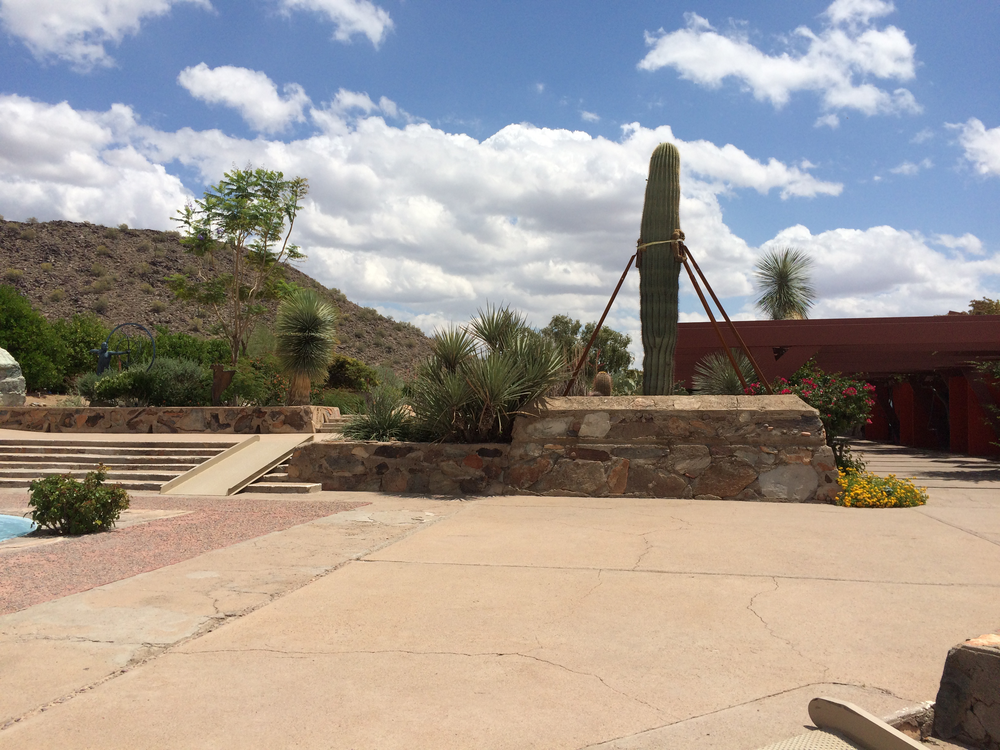
\includegraphics[width=.8\linewidth]{img3_1}
      \caption{Input 1}
    \end{subfigure}
    \begin{subfigure}{.5\textwidth}
      \centering
      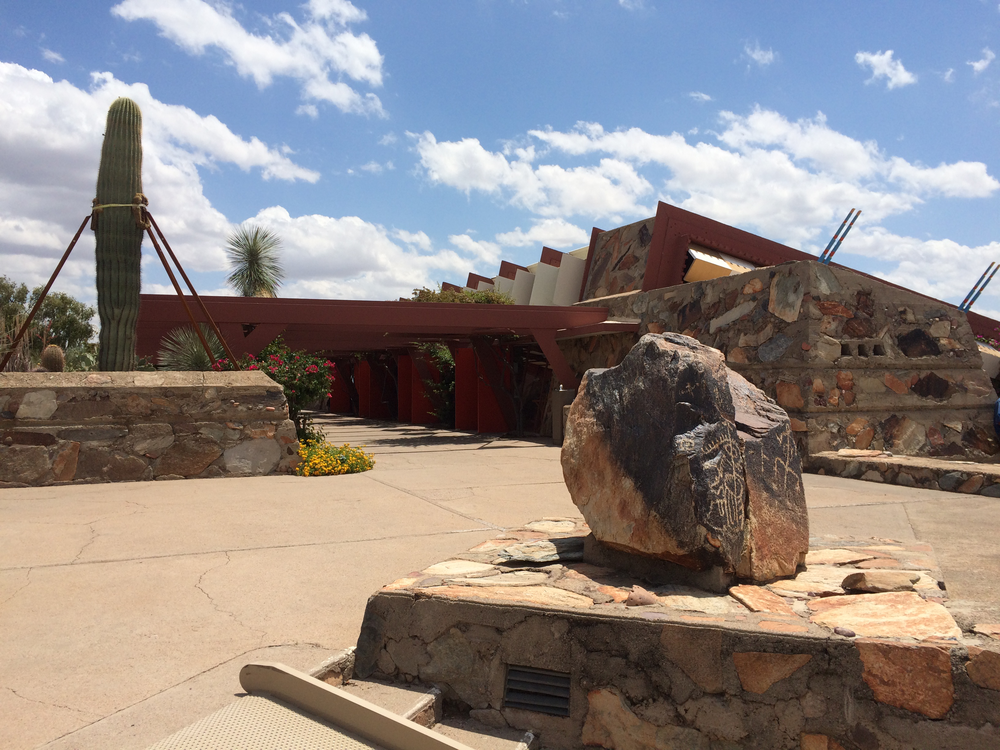
\includegraphics[width=.8\linewidth]{img3_2}
      \caption{Input 2}
    \end{subfigure}
    \begin{subfigure}{\textwidth}
      \centering
      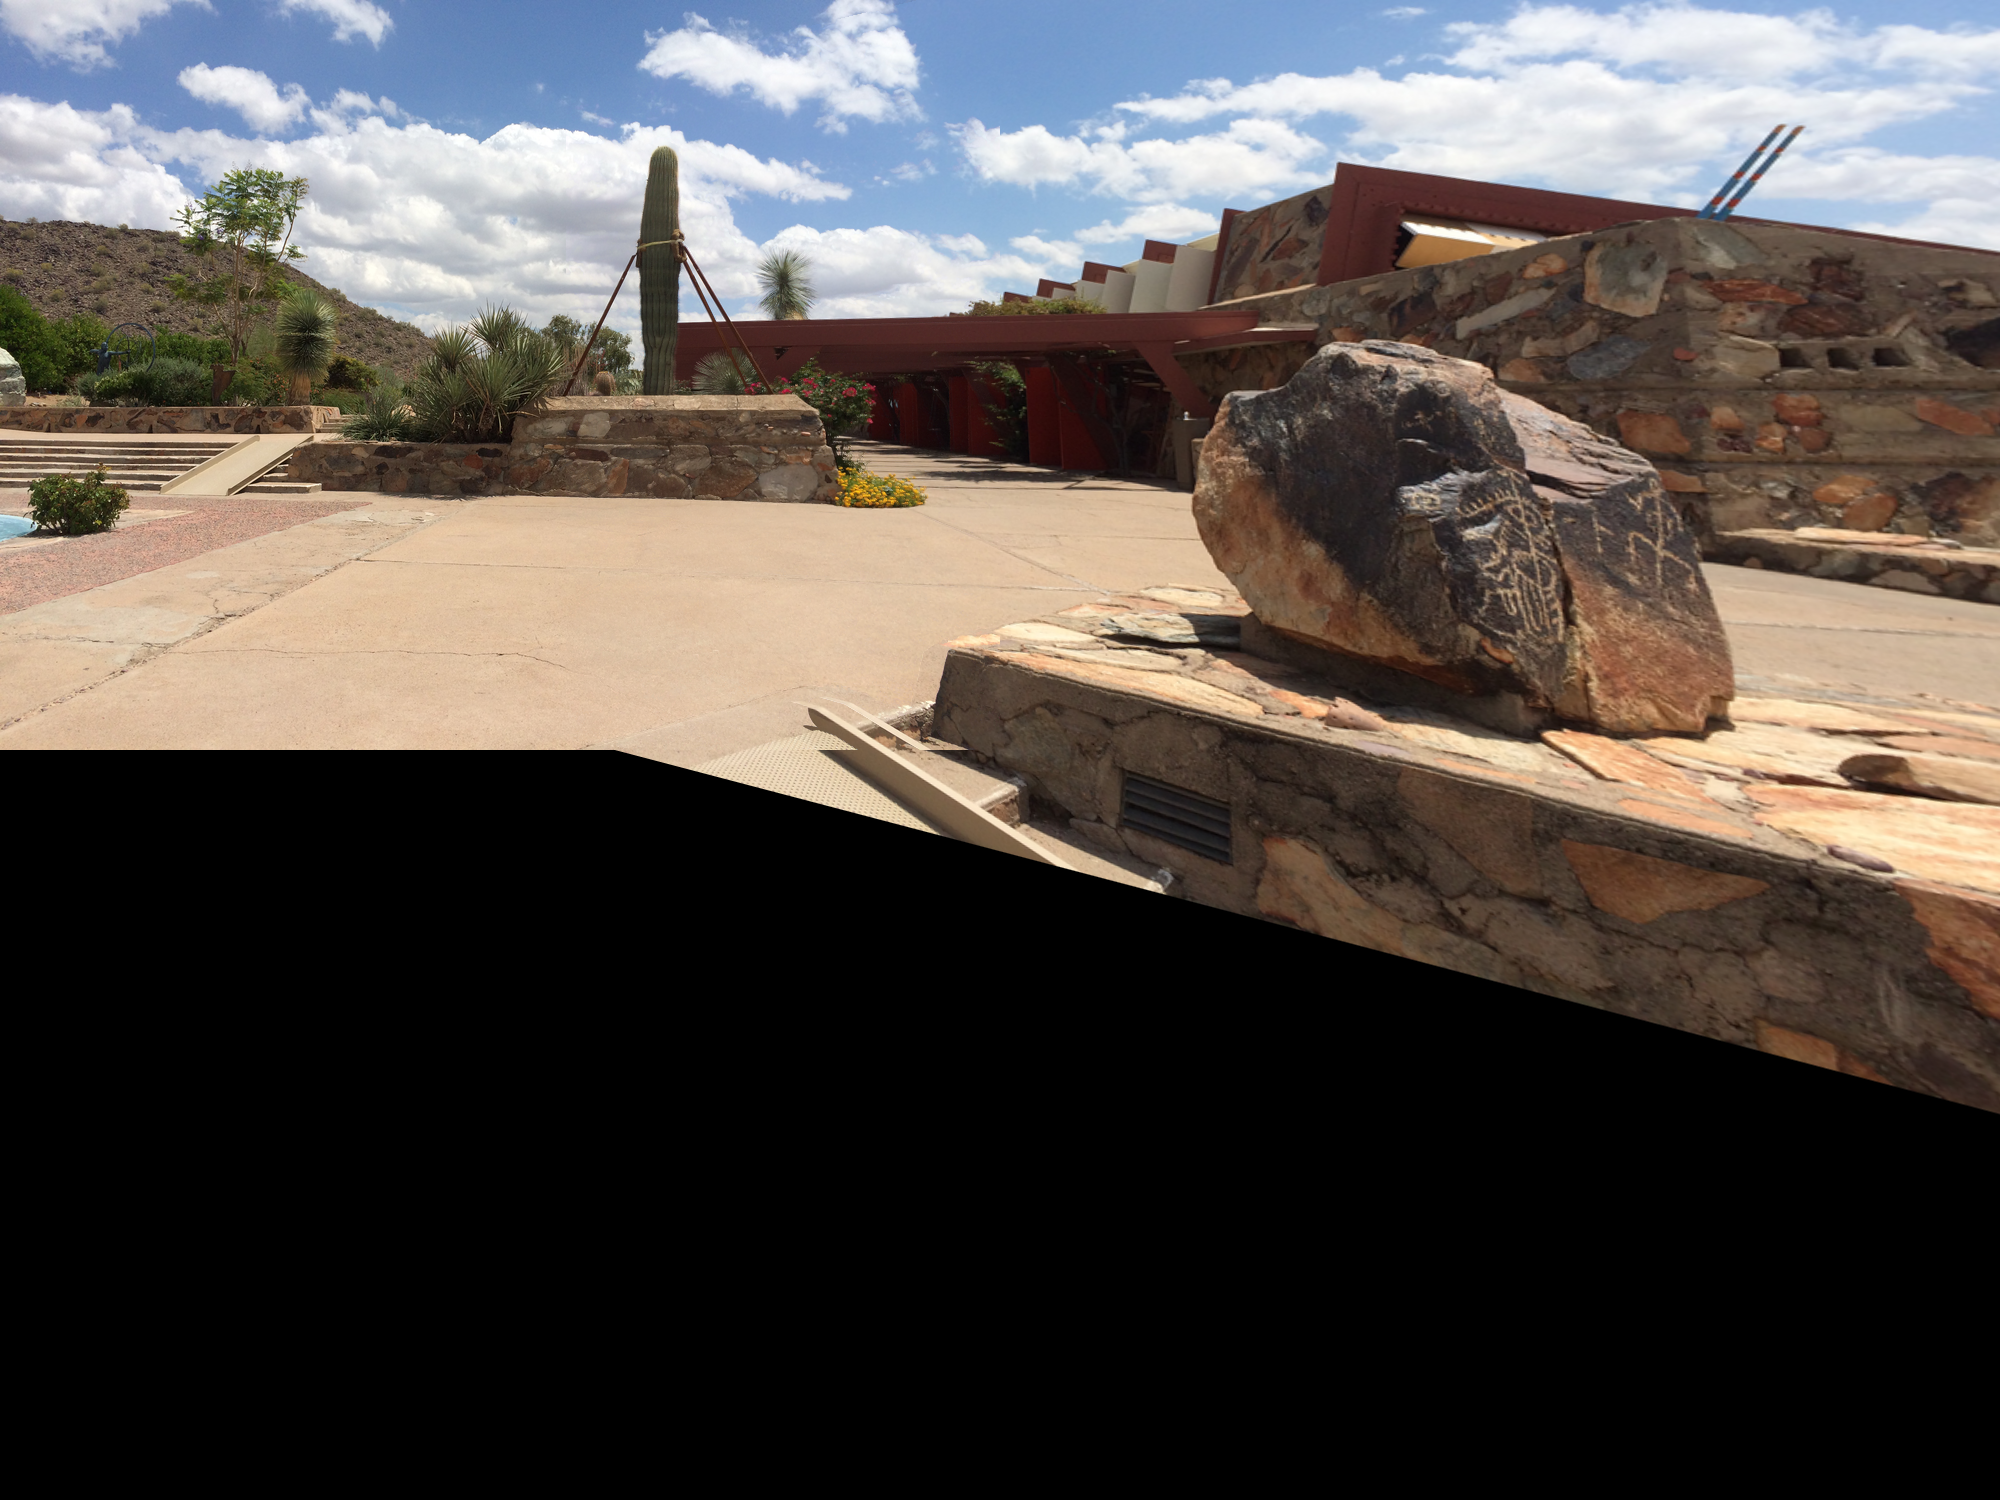
\includegraphics[width=.8\linewidth]{mosaic3}
      \caption{Result}
    \end{subfigure}
  \end{figure}
  \subsection{\texttt{img4} set}
  \begin{figure}[H]
    \begin{subfigure}{.5\textwidth}
      \centering
      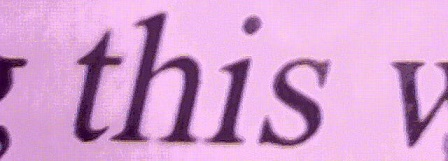
\includegraphics[width=.8\linewidth]{img4_1}
      \caption{Input 1}
    \end{subfigure}
    \begin{subfigure}{.5\textwidth}
      \centering
      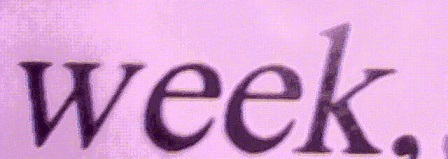
\includegraphics[width=.8\linewidth]{img4_2}
      \caption{Input 2}
    \end{subfigure}
    \end{figure}
    \begin{figure}\ContinuedFloat
    \begin{subfigure}{\textwidth}
      \centering
      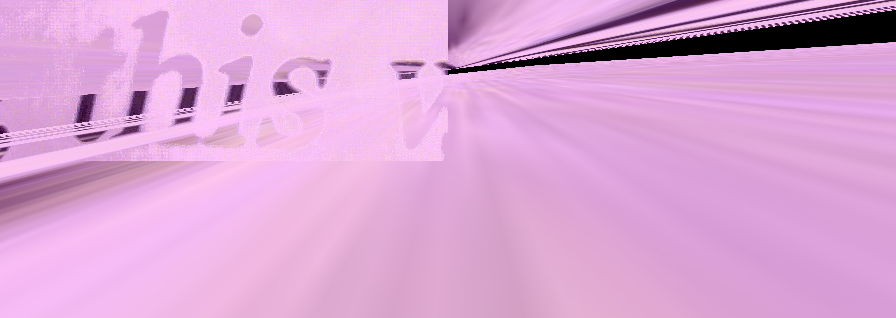
\includegraphics[width=.8\linewidth]{mosaic4}
      \caption{Result}
    \end{subfigure}
  \end{figure}
  
  \begin{figure}[H]
    \centering
    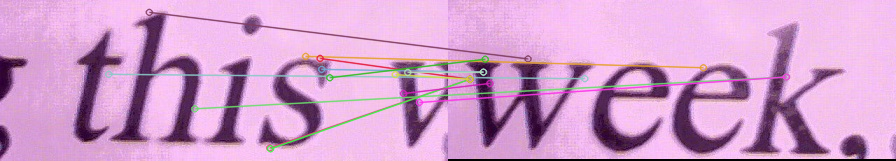
\includegraphics[width=0.8\linewidth]{sift-failure}
    \caption{Except two, none of the matched points are correct and hence the estimated H is incorrect as well. None of the feature descriptors provided in OpenCV - ORB, SURF, etc. - seemed to give better results on this pair of images.}
  \end{figure}
  
  \subsection{Own images}
  
    \begin{figure}[H]
      \begin{subfigure}{.5\textwidth}
	\centering
	\includegraphics[width=.8\linewidth]{img5_1}
	\caption{Input 1}
      \end{subfigure}
      \begin{subfigure}{.5\textwidth}
	\centering
	\includegraphics[width=.8\linewidth]{img5_2}
	\caption{Input 2}
      \end{subfigure}
      \begin{subfigure}{0.5\textwidth}
	\centering
	\includegraphics[width=.8\linewidth]{img5_3}
	\caption{Input 3}
      \end{subfigure}
      \begin{subfigure}{0.5\textwidth}
	\centering
	\includegraphics[width=.8\linewidth]{img5_4}
	\caption{Input 4}
      \end{subfigure}

      \begin{subfigure}{0.5\textwidth}
	\centering
	\includegraphics[width=.8\linewidth]{img5_5}
	\caption{Input 5}
      \end{subfigure}
      \begin{subfigure}{0.5\textwidth}
	\centering
	\includegraphics[width=.8\linewidth]{img5_6}
	\caption{Input 6}
      \end{subfigure}
      
      \begin{subfigure}{\textwidth}
	\centering
	\includegraphics[width=0.5\textwidth]{img5_7}
	\caption{Input 7}
      \end{subfigure}
       \end{figure}
      \begin{figure}\ContinuedFloat
      \begin{subfigure}{\textwidth}
	\centering
	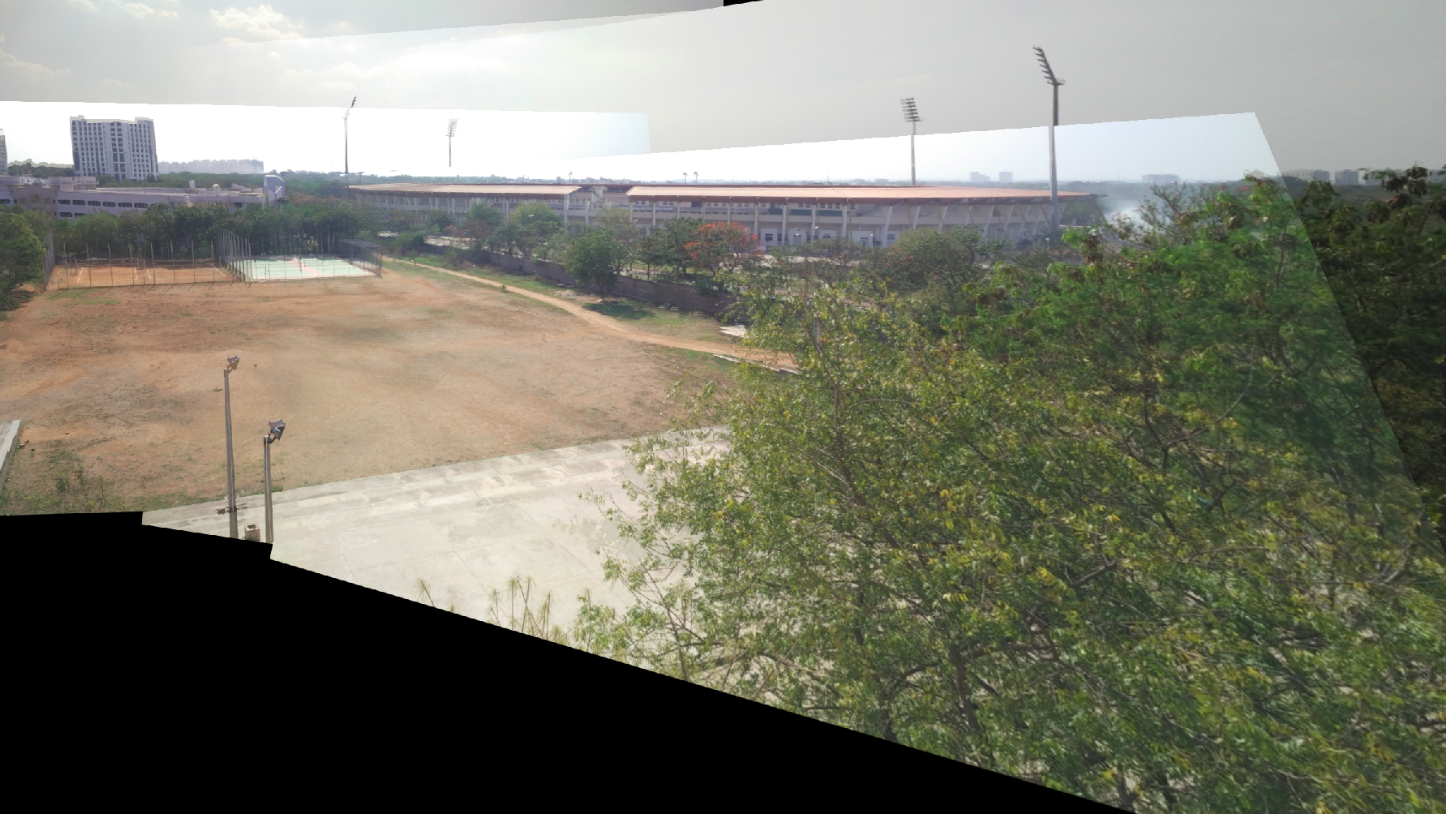
\includegraphics[width=.8\linewidth]{mosaic5}
	\caption{Result}
      \end{subfigure}
      \caption{Felicity ground as seen from Kadamba Nivas 4th floor. Illumination variance across the images and imprecise rotations about the camera center have caused some small deformations in the output mosaic.}
    \end{figure}

\end{document}

